This element simulates a commonplace type of aperture restriction, consisting of a
bump on one or both sides of a chamber. The parameters of the speedbump are
illustrated in Fig. \ref{fig:speedbump}

\begin{figure}[htb]
\center
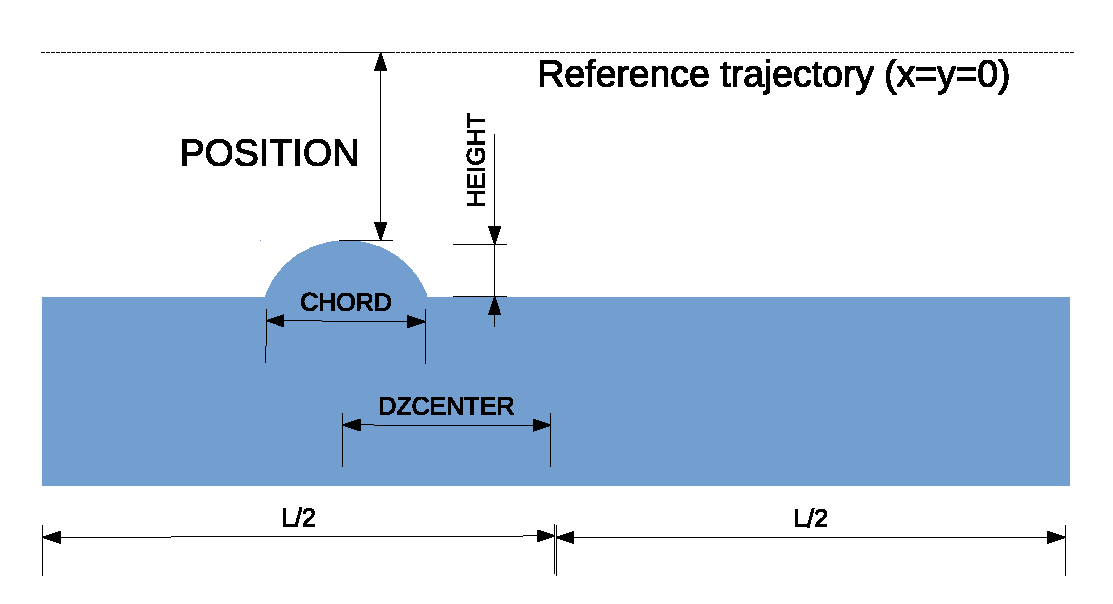
\includegraphics[width=0.8\linewidth]{speedbump}
\caption{Illustration of the parameters used in specifying a speedbump.}
\label{fig:speedbump}
\end{figure}

\clearpage
